\subsection{Practical CSP Algorithms} 
\label{ssec:practical}

We start by defining a more scalable construction of $G^B$.
The augmented graph $G^B$ defined in \cref{ssec:aug} is not a minimal representation as it may contain a lot of redundant information.
For example, the same efficient path $uv$ can be repeated many times in the form $\pp{u,1}\pp{v,0}$, $\pp{u,2}\pp{v,1}$ and so on.
By encoding this information more efficiently, we get considerable improvements both in query time and in data storage.

We construct our \emph{pruned} augmented graph $\Gp^B$ as follows:
As before, nodes are pairs $\pp{v,b}$, but now we add an edge $\pp{v,b}\pp{v',b'}$ only if it is essential for some efficient path, i.e., removing said edge changes the correctness of a query.
If we let $\Pst^E$ be the set of all efficient paths from $s$ to $t$, we take every $P\in \Pst^E$ with cost $b\leq B$ and trace it in the augmented graph such that it terminates at $\pp{t,0}$.
%
%\begin{definition}\label{def:pruned_aug_graph}
%The pruned augmented graph is defined by $\Gp^B=(\Vp^B,\Ep^B)$, where
%\begin{align*}
%\Vp^B &:=\crl{\pp{v,b}: v\in V, b=0,1,\ldots,B},\\
%\Ep^B &:=\crl{\pp{v,b}\pp{u,x} : \exists s,t\in V, P\in\PE_{s,t}, c(P)\leq B, 
% vu\in P, b=c(P[v,t]), x=c(P[u,t]) }.
%\end{align*}
%In $\Gp^B$ all the lengths are preserved.
%\end{definition}
%Note that in $\Gp^B$ there are no sink nodes, hence it has at least $n$ nodes and $nB$ arcs fewer compared to $G^B$.
%In the worst case, those $nB$ arcs are the only gain by doing this process.
%Nevertheless, in our experiments $\Gp^B$ is up to 60\% smaller than $G^B$.
In our experiments $\Gp^B$ is up to 60\% smaller than $G^B$.
For details see \cite{TechReport}.
%Observe that, by running Dijkstra in $G^B$, $\Gp^B$ can be computed in time $\Or(n^2B\log(nB))$.

%\subsubsection{HD of the pruned augmented graph}
%
%A shortest path in $\Gp$ does not necessarily project to an efficient path, even if the path ends in a node of the form $\pp{t,0}$.
%In contrast, if $P$ projects to an efficient path, then necessarily $P$ is shortest. 
%To bound the HD, the correct system to study is
%\[
%\tilde\PB:=\crl{P: P\text{ ends in a node }\pp{t,0}, \bar P\in \PE, c(\bar P)\leq B }.
%\]
%The following result shows how the HD of this system relates to that of $\PE$.
%We omit the proof since it is identical as the one in Proposition~\ref{prop:HDaugmented}.
%\begin{proposition}
%Given CHD $h_c$, the HD of $\tilde\PB$ is $Bh_c$.
%\end{proposition}

\paragraph{Frontier and specific queries}
We test our algorithms with two different tasks.
Recall that the preprocessing is done for some fixed maximum budget $B$.
The first task is a frontier query, wherein given $s$ and $t$, we return the lengths of all efficient paths with costs $b=0,1,\ldots,B$.
The second is called a specific query, for given $s,t,b$ we return $\dist(s,t|b)$, i.e., only one efficient path.
%
%Note that the pruned augmented graph $\Gp^B$ is designed for frontier queries.
%To see this, fix the terminal $\pp{t,0}$.
%As we ask for the shortest path from $\pp{s,B},\pp{s,B-1},\ldots,\pp{s,0}$ we are guaranteed to recover the entire frontier.
%On the other hand, it may be that the shortest path between $\pp{s,b}$ and $\pp{t,0}$ does not correspond to $\dist(s,t|b)$.
%This occurs when $b$ is not a tight budget and the efficient path requires less.
%
%To answer specific queries, we modify $\Gp^B$ by adding extra edges.
%For every $v\in V(G)$ and $b=1,2,\ldots,B$, we include the edge $\pp{v,b}\pp{v,b-1}$ with length $0$.
%A simple argument shows that with the added edges, the shortest path between $\pp{s,b}$ and $\pp{t,0}$ has length $\dist(s,t|b)$.

\paragraph{HL construction via Contraction Hierarchies}
We use some techniques described in \cite{hubimplem} combined with an approach tailored for augmented graphs.
First we give a brief description of Contraction Hierarchies (CH).
Given a ranking of the nodes, which is just a permutation, the CH algorithm proceeds by removing nodes from the lowest rank first.
Whenever a node is removed, we add new edges, called shortcuts, if they are needed to preserve the shortest paths.
Once we have a graph with shortcuts, a CH search is a special variant of Dijkstra; only higher rank nodes are explored, i.e., we never take an edge $uv$ if rank$(u)>\text{rank}(v)$. 

The main idea is to first use contraction hierarchies to get a node ranking and then define the forward hubs of $v$ as the nodes visited during a contraction-based forward search starting at $v$.
The reverse hub is defined analogously.
These are valid hubs, since the highest rank node in a path is guaranteed to be in both hubs.

The most important parameter in CH is the rank; results vary greatly from one choice of ranks to another.
We obtain a rank in $G$ by running a greedy shortest-path cover, which selects the highest rank node as the one covering most uncovered paths in $\PS$ and continues greedily.
%Formally, start with a cover $C=\varnothing$ and compute the set of all shortest paths $\PS$.
%Take a node $v\notin C$ hitting most paths in $\PS$, then remove all those paths from $\PS$, add $v$ to $C$ and iterate.
%The rank is defined as $n$ for the first node added to $C$, $n-1$ for the second and so on.
%To implement the SP cover we follow the algorithm in \cite{hubimplem}.
We stress that this is just an easy way to get a ranking; more sophisticated heuristics that decide on-line the next node to contract usually work well in practice \cite{goldberg_survey,rice_csp}.
Using another contraction scheme may expedite our algorithms and reduce the hub size.

For some instances we work with $G^B$ and for others with $\Gp^B$.
Even though $\Gp^B$ takes some time to compute, it can speed up the overall process and yield considerably better hubs. 
Given a rank for nodes in $G$, we contract $\Gp^B$ as follows.
Say that $V$ is ordered according to the rank, so node~$1$ is the least important and $n$ the most important.
In $\Gp^B$, we first contract the nodes $\pp{1,b}$ for $b=B,\ldots,0$, then the nodes $\pp{2,b}$ and so on till the nodes $\pp{n,b}$ are the last to contract. 
Finally, when contracting a node $v$, if $u$ is a predecessor and $w$ a successor of $v$, one should add the short-cut $uw$ only if, by removing $v$, the distance from $u$ to $w$ is altered.
We can go even further; the short-cut $uw$ is unnecessary if the shortest path is not efficient, even if the distance changes.
To obtain better hubs we prune the results obtained by CH with additional techniques, for details see \cite{TechReport}.
%If $w$ is in the forward search of $v$ with distance $d$, it might be that $\dist(v,w)<d$, this occurs because the search goes only to higher rank nodes and the discovered path is missing some node.
%When $\dist(v,w)<d$, we can safely remove $w$ from the hub of $v$, since the highest ranked node in a shortest path will have the correct distance.
%For frontier queries, we can also prune away a node $w$ if the $(v,w)$-path has a surplus of budget.
%The entire process can be summarized in the following steps.

\begin{table*}
\resizebox{\textwidth}{!}{%
\begin{tabular}{| l | p{1cm} | p{1cm} | p{1cm} | p{1.2cm} | p{1.2cm} | }
\hline
	B & Prepro [m] & Avg F Size & Avg B Size & Query Dij [ms] & Query HL [ms] \\ \hline \hline
	0 & 1 & 23 & 22 & 10.71 & 0.005 \\ \hline
5-f  & 5  & 16 & 28 & 80.10  & 0.02 \\
5-s  & 5  & 57 & 28 & 31.75  & 0.01 \\ \hline
10-f & 9  & 9 & 28 & 168.11 & 0.03 \\
10-s & 10 & 68 & 28 & 56.19  & 0.01 \\ \hline
%15-f & 12 & 6 & 28 & 237.64 & 0.03 \\
%15-s & 16 & 73 & 28 & 77.59  & 0.01 \\ \hline
20-f & 17 & 5 & 28 & 342.47 & 0.03 \\
20-s & 20 & 77 & 28 & 100.26 & 0.01 \\ \hline
%25-f & 22 & 4 & 28 & 460.95 & 0.03 \\
%25-s & 25 & 80 & 28 & 126.52 & 0.01 \\ \hline
30-f & 26 & 3 & 28 & 569.13 & 0.03 \\
30-s & 31 & 84 & 28 & 152.75 & 0.01 \\ \hline
\end{tabular}
\quad
\begin{tabular}{ | l | p{1cm} | p{1cm} | p{1cm} | p{1.2cm} | p{1.2cm} |}
\hline
	B & Prepro  [m] & Avg F Size & Avg B Size & Query Dij [ms] & Query HL [ms] \\ \hline \hline
	0 & 6 & 18 & 18 & 16.35 & 0.004 \\ \hline
5-f  & 1  & 18.0 & 18.0 & 175.04  & 0.02 \\
5-s  & 21 & 42.9 & 18.7 & 72.03   & 0.01 \\ \hline
10-f & 2  & 18.0 & 18.0 & 361.15  & 0.04 \\
10-s & 35 & 49.3 & 18.7 & 102.52  & 0.01 \\ \hline
%15-f & 3  & 18.0 & 18.0 & 577.89  & 0.06 \\
%15-s & 46 & 53.3 & 18.7 & 140.80  & 0.01 \\ \hline
20-f & 4  & 18.0 & 18.0 & 821.94  & 0.07 \\
20-s & 60 & 56.5 & 18.7 & 183.11  & 0.01 \\ \hline
%25-f & 5  & 18.0 & 18.0 & 974.84  & 0.09 \\
%25-s & 77 & 59.5 & 18.7 & 227.17  & 0.01 \\ \hline
30-f & 7  & 18   & 18   & 1247.72 & 0.10 \\
30-s & 93 & 62.3 & 18.7 & 272.41  & 0.01 \\ \hline
\end{tabular}%
}
\vspace{13pt}
\caption{Experimental results for San Francisco (left) and Luxembourg City (right). Query times are measured with 1000 random $s,t$ pairs for each network and multiple maximum budget levels $B$. Results on rows $B-f$ correspond to computing the solution frontier for all budgets $b\leq B$ while rows $B-s$ correspond to computing the solution for budget level $b$.}
\label{tab:performance_results}
\end{table*}


%\begin{enumerate}[nosep]
%\item Compute the shortest paths in $G$ and use a greedy approach to obtain a cover $C$
%\item Compute the pruned augmented graph $\Gp^B$
%\item Contract $\Gp^B$ using the rank induced by $C$
%\item Create hubs $\Lf(v),\Lb(v)$ using CH
%\item Prune the hubs by running HL queries between $v$ and nodes in $\Lf(v)$. 
%Run a similar process for $\Lb(v)$.
%\end{enumerate}
%Recall that, for some instances, we skip step 2 and contract $G^B$ instead.
%Note that in the last step we bootstrap HL to improve it.
%This works because the fact that some nodes have incorrect distance labels does not impact the correctness of a HL query; a node minimizing the distance is returned and such node must have a correct label.

\begin{figure}
\begin{minipage}{0.25\textwidth}
\centering
\begin{tikzpicture}[trim axis left]
\begin{axis}[
	scale only axis,
	height=3cm,
	width=3.9cm,
	xtick distance=300,
	ytick distance=1,	
	xmin = 10, xmax =1000,
	xlabel={Number of clusters},
	ylabel={},
	every axis plot/.append style={thick}]
\addplot[mark size=0.3,draw=black, mark=square*] table {tab_avg_sf.dat};
\addplot[mark size=0.3,draw=red, mark=triangle*] table {tab_max_sf.dat};
\addplot[mark size=0.3,draw=blue, mark=diamond*] table {tab_shorts_sf.dat};

\legend{Avg hub size, Max hub size,\# shortcuts}
\end{axis}
\end{tikzpicture}

\end{minipage}%
\begin{minipage}{0.25\textwidth}
\centering
\begin{tikzpicture}[trim axis left]
\begin{axis}[
	scale only axis,
	height=3cm,
	width=3.9cm,
	xtick distance=300,
	ytick distance=1,	
	xmin = 10, xmax =1000,
	xlabel={Number of clusters},
	ylabel={},
	every axis plot/.append style={thick}]
\addplot[mark size=0.3,draw=black, mark=square*] table {tab_avg_lu.dat};
\addplot[mark size=0.3,draw=red, mark=triangle*] table {tab_max_lu.dat};
\addplot[mark size=0.3,draw=blue, mark=diamond*] table {tab_shorts_lu.dat};

\legend{Avg hub size, Max hub size,\# shortcuts}
\end{axis}
\end{tikzpicture}

\end{minipage}
\caption{Performance of clustering for San Francisco (left) and Luxembourg (right). 
In the $y$-axis the quantities are normalized by the best greedy cover, i.e., using $k=n$.
Note that, while the number of short-cuts is an indicator of performance, it is not perfectly correlated with the hub size.}
\label{fig:clusters}
\end{figure}

\vspace{-0.5em}
\begin{remark}
To compute a shortest path cover, a direct approach requires storing all the shortest paths in memory.
In many cases, this can impose a prohibitive memory requirement.
There are two ways around this issue.
We can compute the cover by processing one shortest path tree at a time, this translates to $\Omega(n^3\log n)$ running time, but $\Or(n)$ memory.
The second approach we suggest is to compute only $k<<n$ shortest path trees and cover these greedily.
We use an off-the-shelf clustering method to obtain $k$ cluster centers, from which we compute the shortest paths. 
As shown in Figure~\ref{fig:clusters}, the clustering approach provides a very good approximation of the hubs with even a small $k$.
\end{remark}

\subsection{Experiments} 
\label{sec:exp}

All our experiments were performed on a 64-bit desktop computer with a 3.40GHz Intel Core i7-6700 processor and 16GB RAM running Ubuntu 16.04.
Our code is written in Python 2.7.
We use the library Networkx for the graph representation and Dijkstra's algorithm.
Although all the steps can be parallelized, we did not implement this.
The code is available at (hidden for anonymity).%\url{github.com/albvera/HHL_CSP}.

We evaluated the performance of our algorithms with real-world test networks: a downtown San Francisco network with 2139 nodes and 5697 edges for which real-world travel-time data was available as a Gaussian mixture model \cite{sf_data}, and a Luxembourg City network with 4026 nodes and 9282 edges for which travel-time distributions were synthesized from speed limits \cite{niknami2016tractable}, as real-world data was unavailable.
 
In our experiments, we use the mean travel times for our length function and the following cost structure; the top 10\% of edges with the highest variance are assigned cost 1 and the rest cost 0.
This is a measure of risk, since edges with high variance are prone to cause a delay in the travel time.


\begin{figure*}
\resizebox{\textwidth}{!}{%
\begin{minipage}[t]{.29\textwidth}
\centering
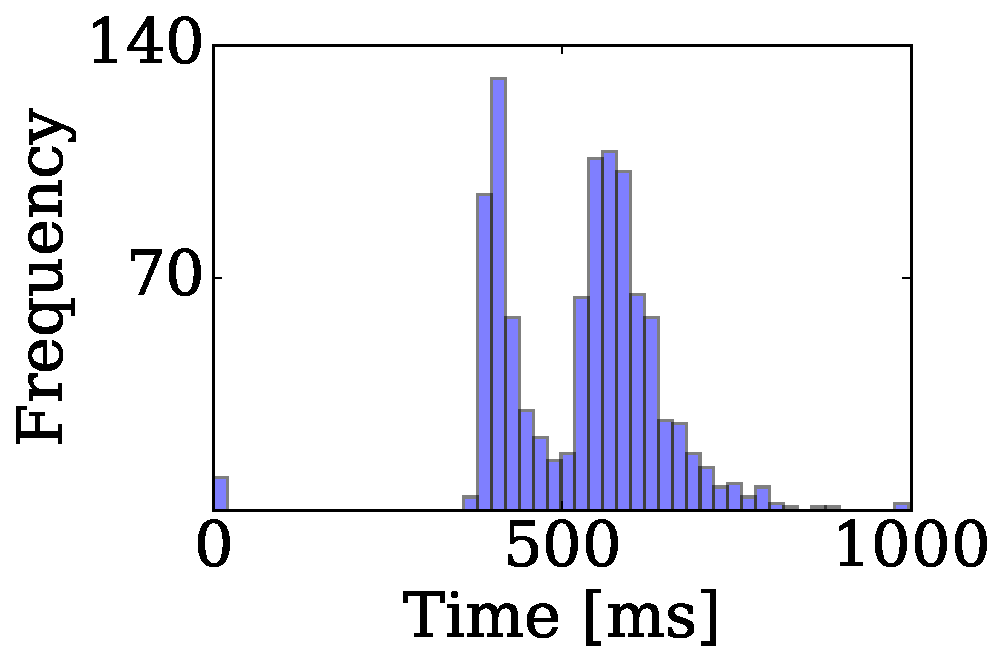
\includegraphics[clip, trim=0.2cm 0.3cm 0.4cm 0.2cm,scale=0.3]{TexImg/SF_query_dij_B25.pdf}
(a)
\end{minipage}
\begin{minipage}[t]{.25\textwidth}
\centering
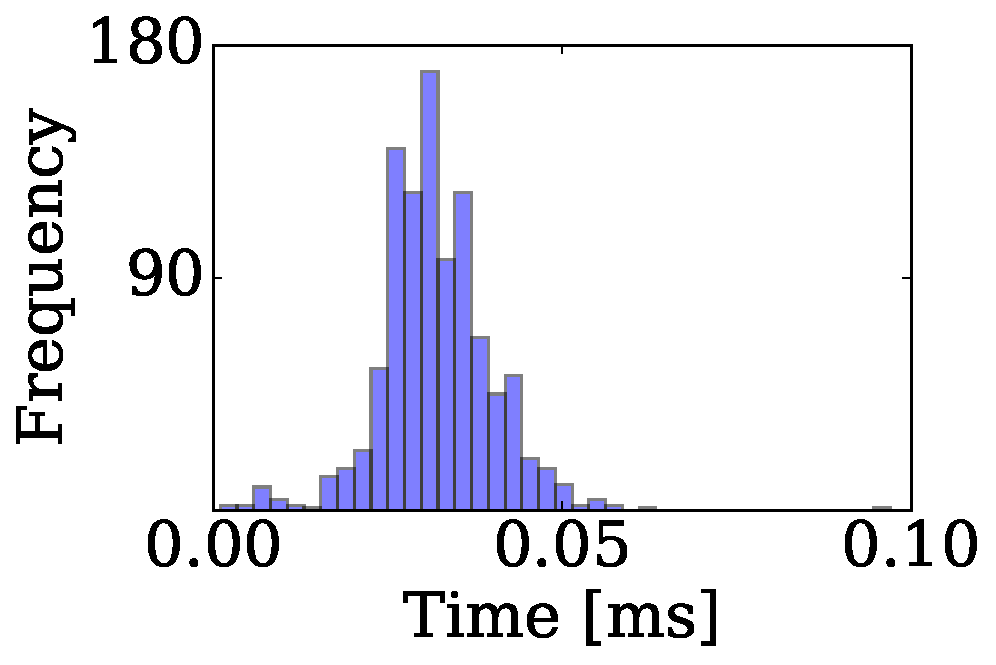
\includegraphics[clip, trim=1.3cm 0.3cm 0.2cm 0.2cm,scale=0.3]{TexImg/SF_query_hl_B25.pdf}
(b)
\end{minipage}
\begin{minipage}[t]{.25\textwidth}
\centering
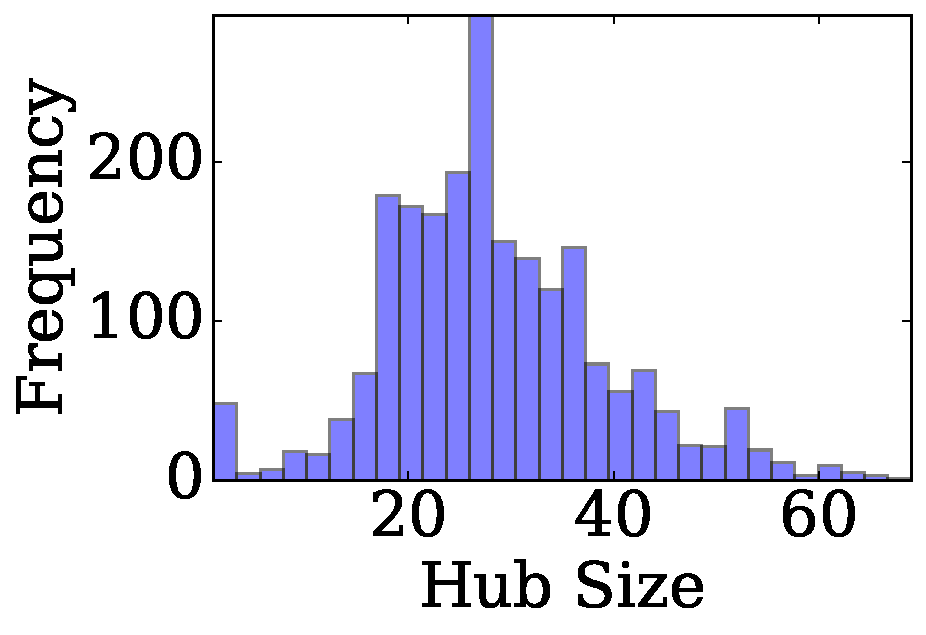
\includegraphics[clip, trim = 1.3cm 0.3cm 0cm 0cm,scale=0.3]{TexImg/SF_bwd_hub_size.pdf}
(c)
\end{minipage}
\begin{minipage}[t]{.25\textwidth}
\centering
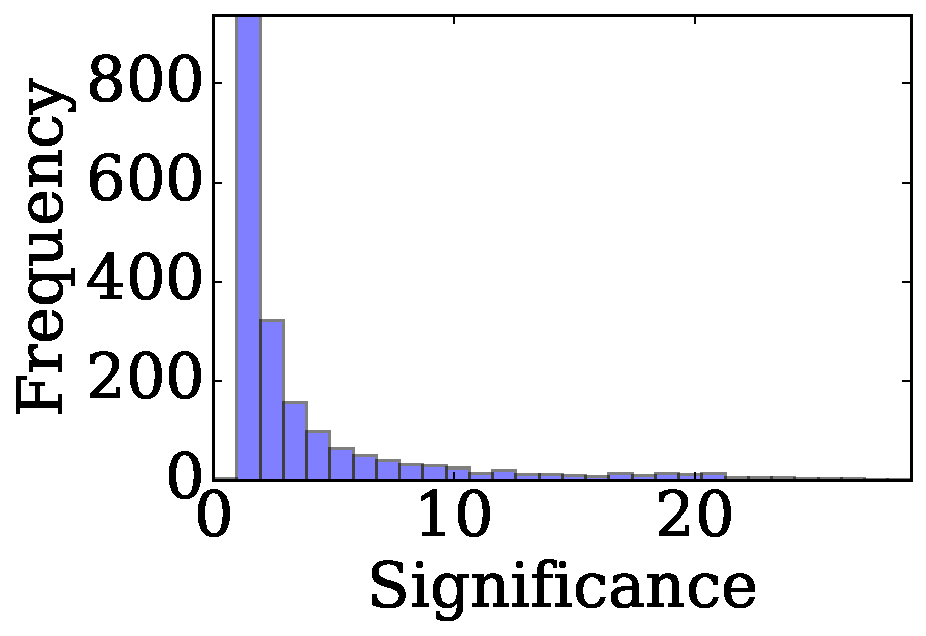
\includegraphics[clip, trim = 1.3cm 0.3cm 0cm 0cm,scale=0.3]{TexImg/significance.pdf}
(d)
\end{minipage}
}
\caption{ Histogram frontier queries for Dijkstra (a) and HL (b). Times are 1000 random pairs in San Francisco augmented with $B=25$.
Size of reverse hubs (c) and significance (d) for frontier queries in San Francisco augmented with $B=25$.
}
\label{fig:SF_query}
\label{fig:SF_bwd_size}
\end{figure*}

\paragraph{Query-time performance}
Table~\ref{tab:performance_results} presents the CSP computation times for different maximum budgets $B$. 
For frontier queries, labelled as `f', the query times are measured as the average of 1000 random $s,t$.
For specific queries, labelled as `s', the times are measured as 1000 random triplets $s,t,b$.
The column for $B=0$ represents the original graph (without augmentation). 
As can be seen in the experimental results, our method finds the constrained shortest path solution on average four orders of magnitude faster than running Dijkstra's algorithm on the augmented graph. 
Preprocessing for frontier queries results in a more compact set of hub labels, since a node $\pp{s,b}$ needs to store information for paths with budget exactly equal to $b$ (in case the path is efficient, otherwise it is not stored).
On the other hand, for specific queries, $\pp{s,b}$ needs to store information for all budgets up to $b$.
The preprocessing time does not include the cover computation, since this is a flat cost of at most the time to preprocess the instance $B=0$.

Note that preprocessing frontier queries in Luxembourg is faster, despite the network being bigger, this can be explained by the structural properties.
For example, in Luxembourg there are more highways and fast roads.
Observe that the \emph{average hub size decreases} in San Francisco, this is because in this instance we use $\Gp$, which prunes away most of the nodes, thus many nodes $\pp{v,b}$ are isolated and have empty hubs.
The longer preprocessing time for frontier queries can be explained as follows.
There are many cases when two nodes are not reachable, to detect this requires Dijkstra to explore the entire graph.
In contrast, for specific queries we add extra edges $\pp{s,b}\pp{s,b-1}$, hence a reachability test ends, in average, earlier.
In the contraction step, we want to remove a node without altering the shortest path, a process that requires many reachability tests.


\paragraph{Hub sizes and node significance}
We focus the analysis on two meaningful quantities.
The first is hub size, which is well captured by  $\card{\Lb(\pp{t,0})}$ for $t\in V$.
Indeed, for frontier queries the reverse hub is bounding the space requirements; for specific queries the same is true up to a constant factor.
For the second quantity, we define the significance of $s\in V$ as the number of hubs containing $s$, i.e., $\sum_t\sum_b\In{\pp{s,b}\in \Lb(\pp{t,0})}$.
Intuitively, a node is highly significant if belongs to many efficient paths.
Figure~\ref{fig:SF_bwd_size} shows a histogram of these metrics. 

	
%\begin{figure}
%\begin{minipage}[t]{.51\textwidth}
%\centering
%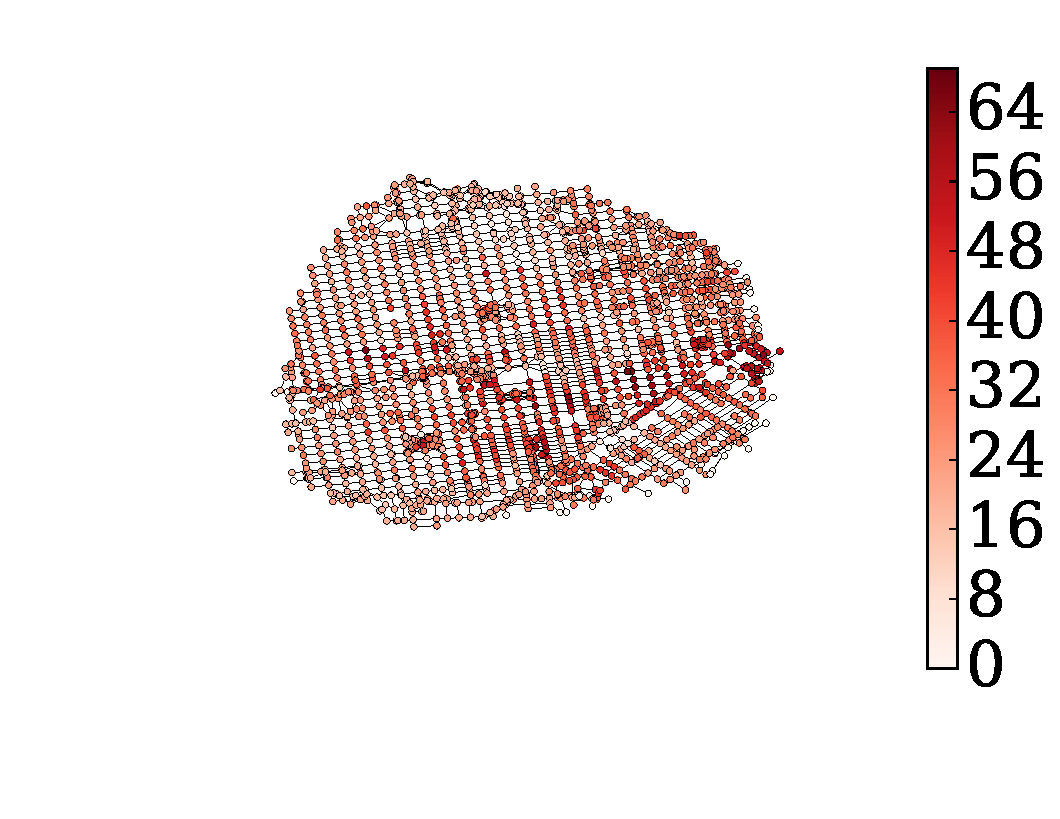
\includegraphics[clip, trim=4.5cm 4.8cm 4.7cm 3cm,height=4.5cm]{TexImg/SF_hub_sizes.pdf}
%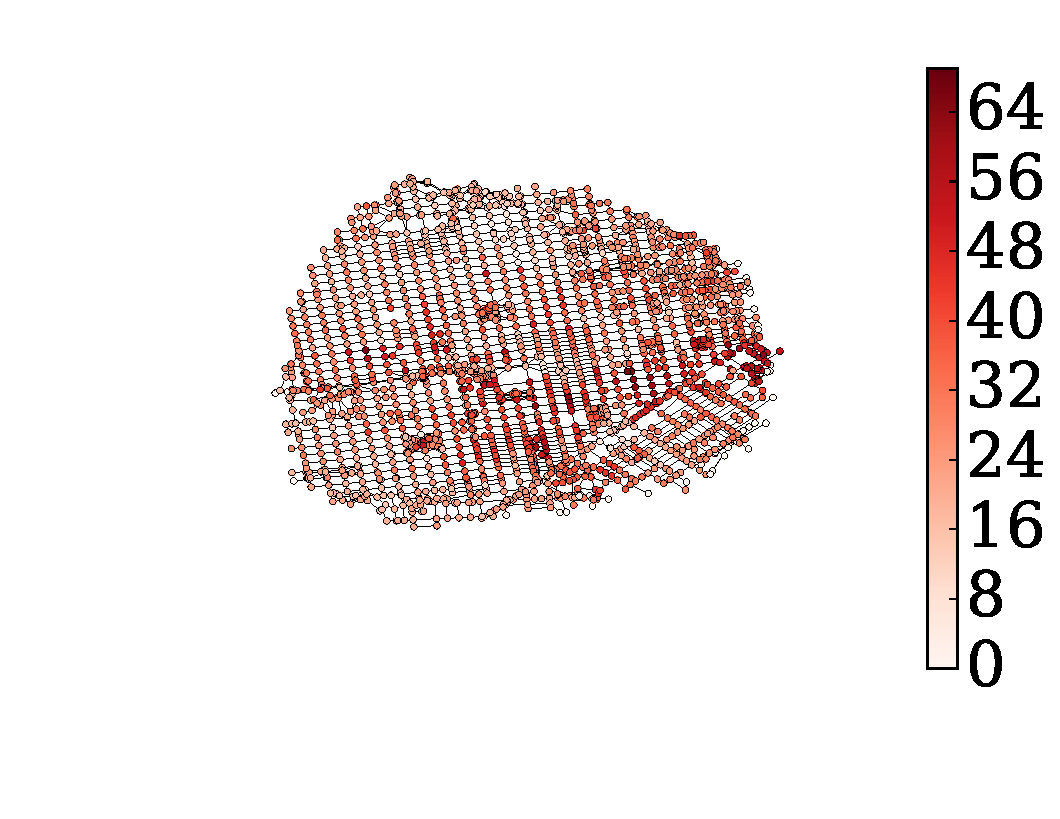
\includegraphics[clip, trim=15.8cm 0cm 0.4cm 1cm,scale=0.3]{TexImg/SF_hub_sizes.pdf}
%\caption{Heat map of hub size for frontier queries in San Francisco augmented with $B=25$.
%Note that the size is not homogeneous, but rather we can observe clusters and neighborhoods tend to be similar.}\label{fig:SF_hub_size_map}
%\end{minipage}
%\hfill
%\begin{minipage}[t]{.46\textwidth}
%\centering
%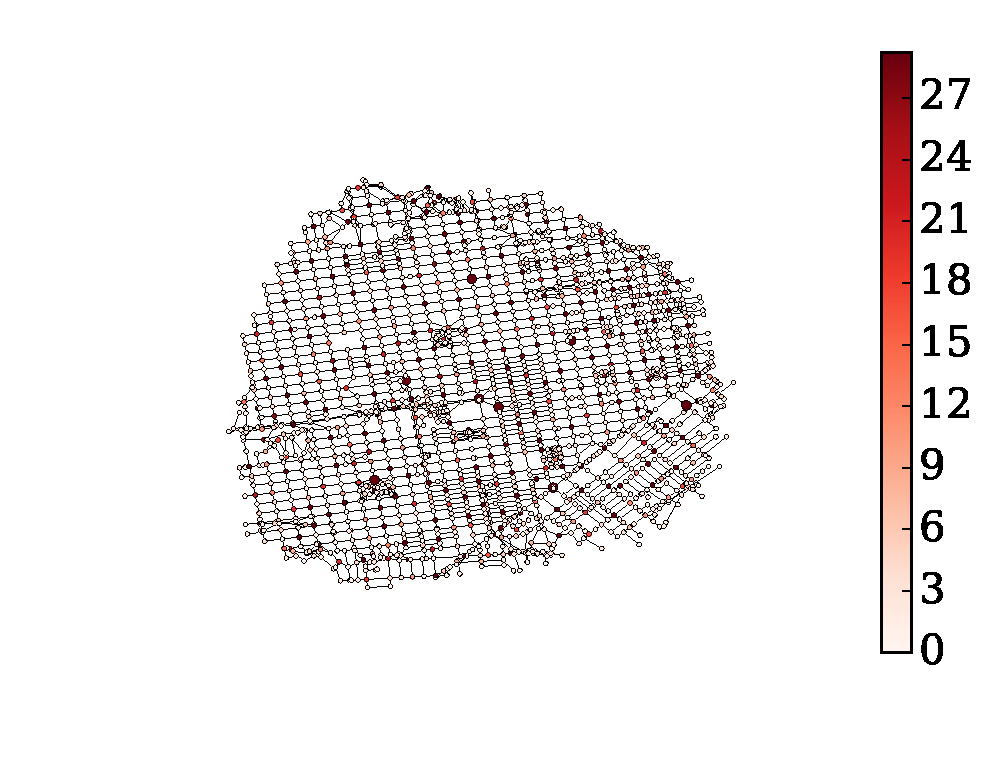
\includegraphics[clip, trim=3.7cm 2.9cm 4.2cm 3cm,height=4.5cm]{TexImg/sig_colapse.pdf}
%%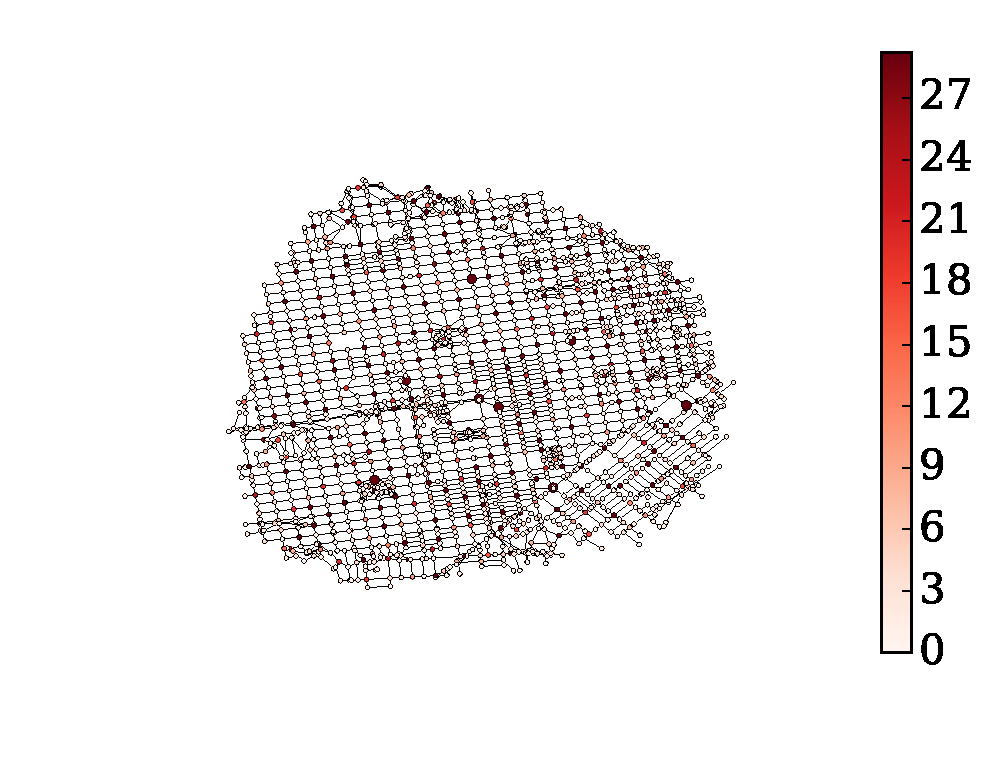
\includegraphics[clip, trim=15cm 1.5cm 0.1cm 0.8cm,scale=0.45]{TexImg/sig_colapse.pdf}
%\caption{Heat map of significance for frontier queries in San Francisco augmented with $B=25$.
%The most significant nodes have been drawn bigger.
%The top 3 most significant correspond to Geary Blvd \& Gough St, Franklin St \& O'Farrel St and Market St \& Polk St.}
%\label{fig:sig_colapse}
%\end{minipage}
%\end{figure}

Figures \ref{fig:SF_hub_size_map} and \ref{fig:sig_colapse} show the spatial relationships between the hub size and significance in the San Francisco network. 
We observe that highly significant nodes tend to have small hub size.
The intuition is simple, if most hubs contain $s$, then is easier for $s$ to satisfy the cover property with a small hub.
Note also that the hub size resembles an harmonic function; nodes are mostly similar to their neighbors.

\begin{figure}
\begin{minipage}[t]{.53\textwidth}
\centering
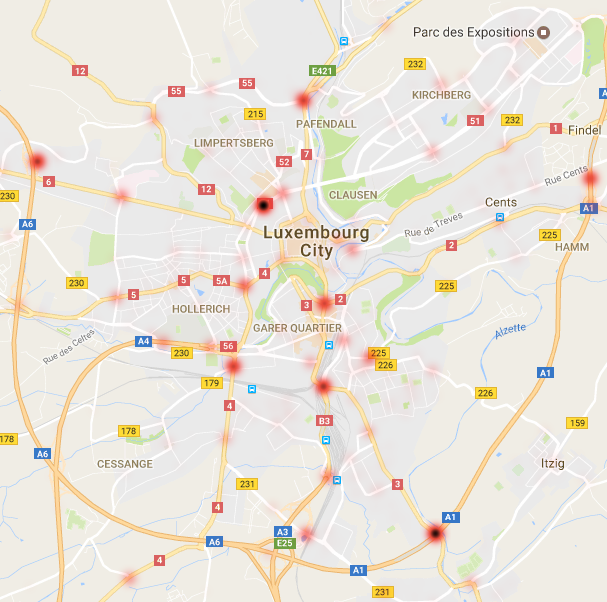
\includegraphics[scale=0.3]{TexImg/map_LU_sig.png}
\caption{Heat map of significance for frontier queries in Luxembourg City augmented with $B=25$.
Notice how the highly significant nodes are in main road crossings.}
\label{fig:map_LU} 
\end{minipage}
%\hfil
%\begin{minipage}[t]{.43\textwidth}
%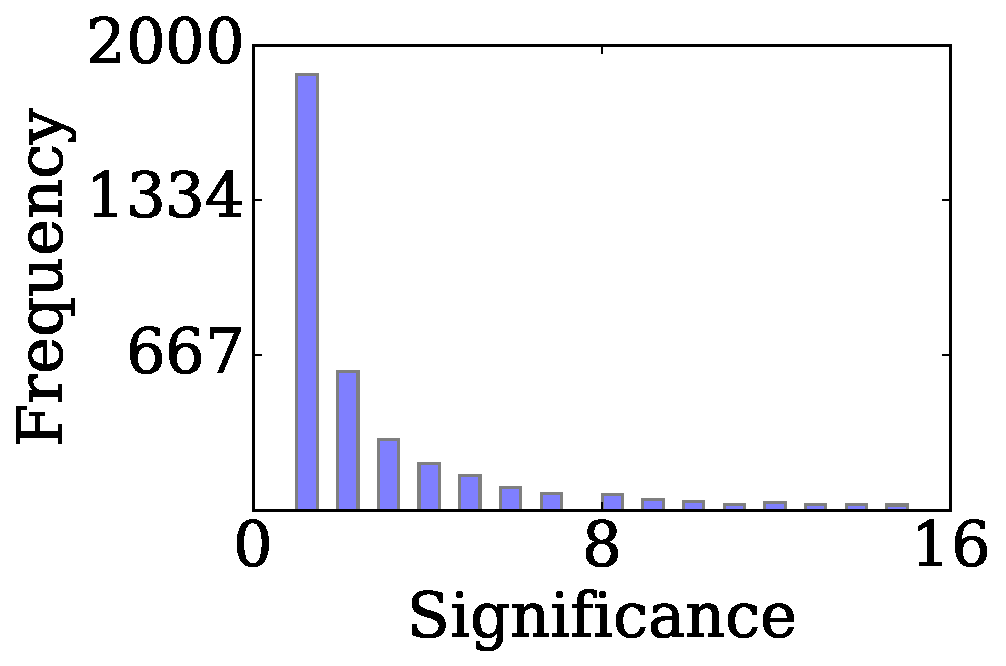
\includegraphics[scale=0.35]{TexImg/significance_LU.pdf}
%\caption{Histogram of significance in Luxembourg City augmented with $B=25$.
%The top 10\% most significant nodes were out of scaled and have been collapsed for exposition purposes.}
%\label{fig:sig_LU} 
%\end{minipage}
\end{figure}